\begin{tikzpicture}[font = \Large]
  \node (share) [label = {below:共享数据}] {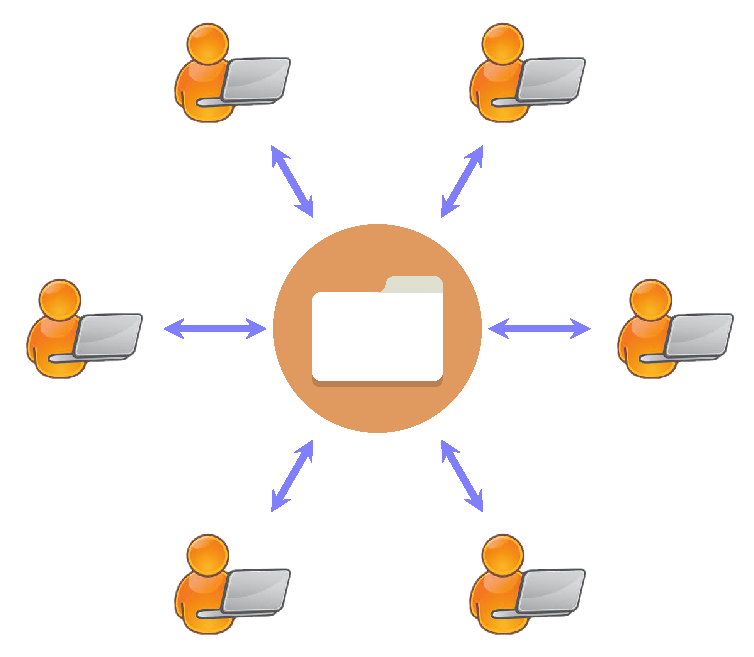
\includegraphics[height = 4cm]{shared-data-clients.pdf}};
  \node (dist) [label = {below:分布数据}, right = 9.0cm of share] {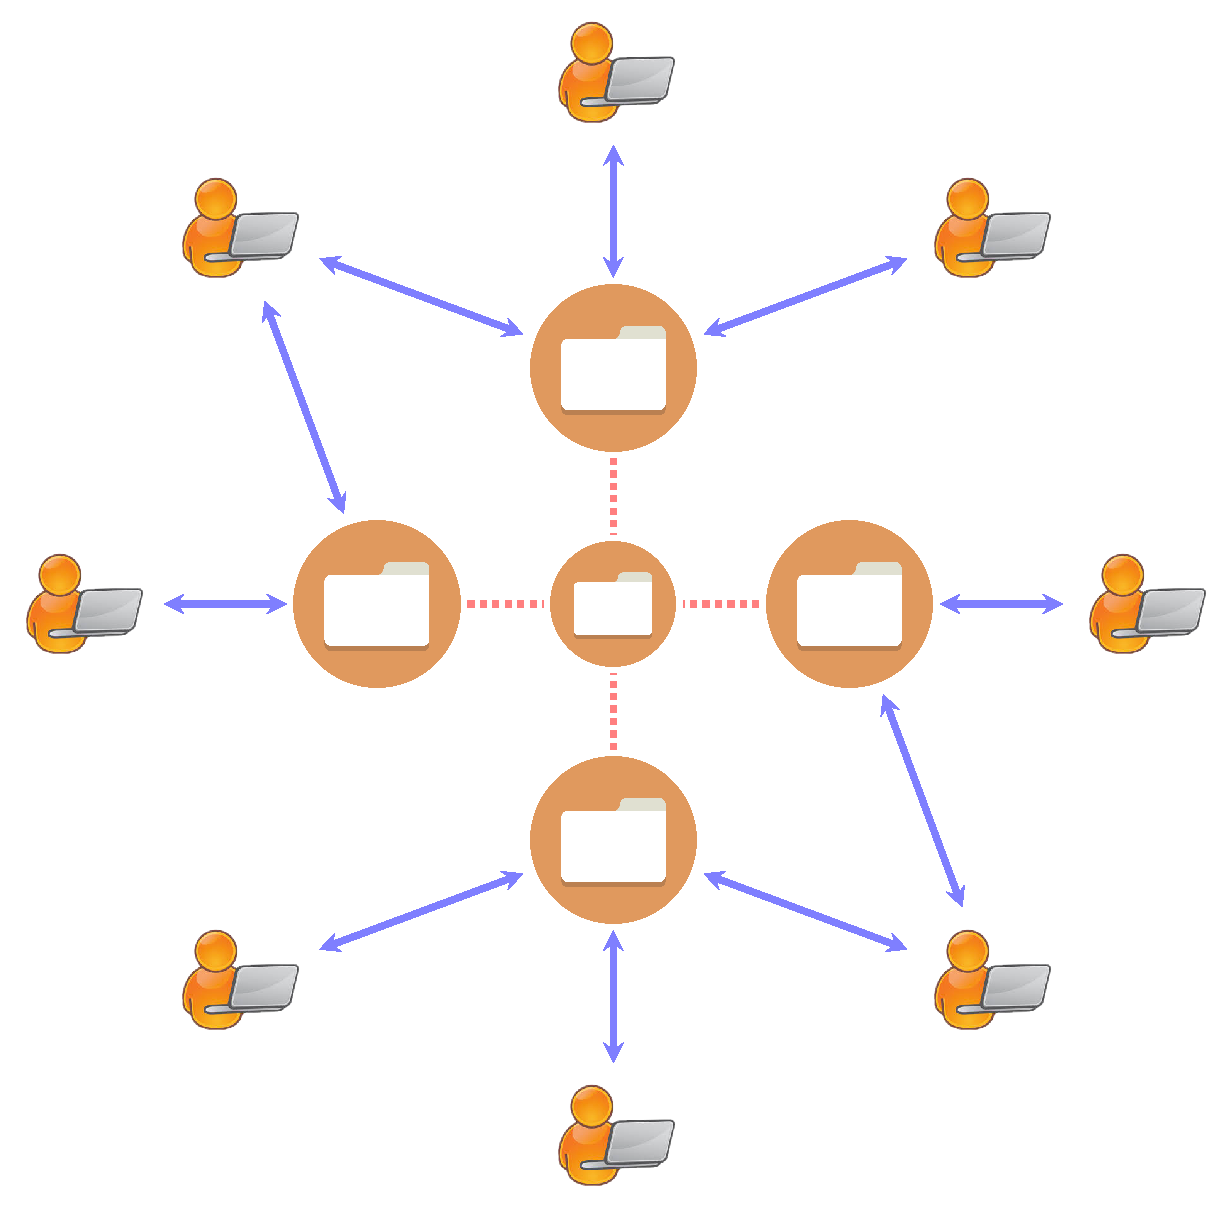
\includegraphics[height = 4.5cm]{distributed-data-clients.pdf}};

  % from (share) to (dist)
  \uncover<2->{
  \draw [-Implies, brown, line width = 1pt, double distance = 2pt, bend right = 35] (share) to node [black, sloped, below = 8pt] {分布数据一致性问题} (dist);
  }

  % from (dist) to (share)
  \uncover<4->{
  \draw [-Implies, brown, line width = 1pt, double distance = 2pt, bend right = 35] (dist) to node () [black, sloped, above = 8pt] 
  {像访问共享数据一样访问分布数据} (share);
  }

  % middleware
  \uncover<3->{
  \node (dsds) [] at ($(share.center)!0.5!(dist.center)$) {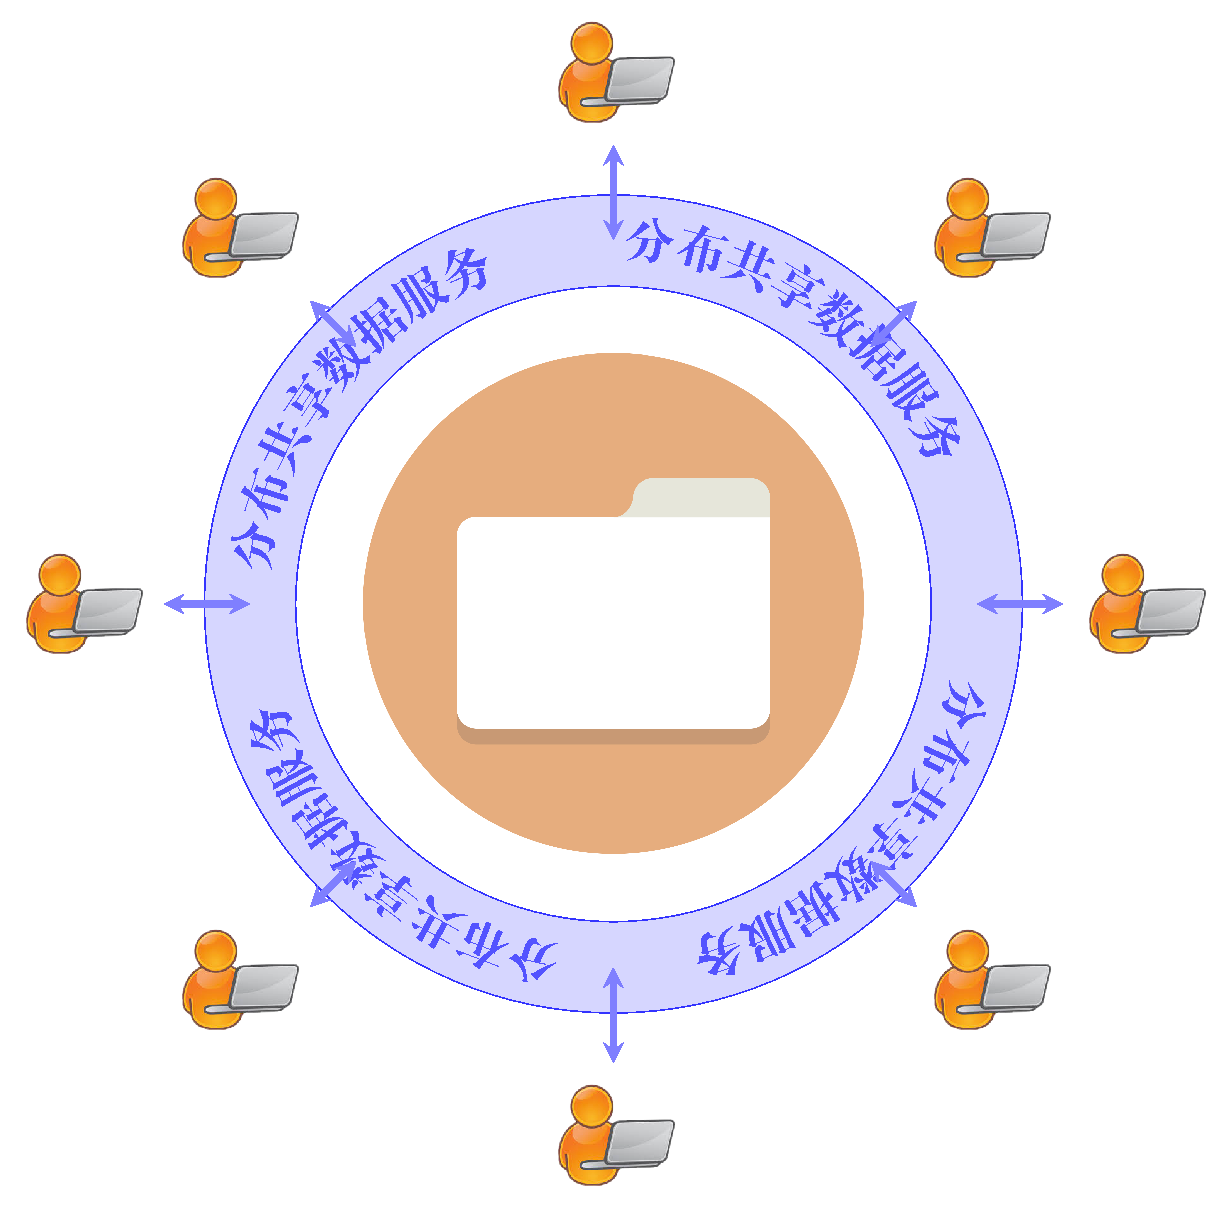
\includegraphics[height = 6cm]{distributed-shared-data-clients-chinese.pdf}};
  \draw [-Implies, blue!60, line width = 1pt, double distance = 1pt] (dist) to (dsds);
  \draw [-Implies, blue!60, line width = 1pt, double distance = 1pt] (dsds) to (share);
  }
\end{tikzpicture}